\section{Architettura}
L'architettura del prodotto si basa su un modello di comunicazione tra Client e Server, all'interno della quale possiamo trovare i seguenti componenti: 
\begin{itemize}
    \item \glossario{Client}: interfaccia web realizzata utilizzando \glossario{React} che permette all'utente di interfacciarsi con i servizi offerti dal chatbot. 
    \item \glossario{Server}: si occupa di gestire le richieste in arrivo dai client, contattando le API-Rest offerte da Imola per svolgere le operazioni
    \item API \glossario{Rest} Imola Informatica: insieme dei servizi resi disponibili dall'azienda, vengono contattate dal server ed effettuano la richiesta a cui sono associate.  
\end{itemize}

\subsection{Client}
\subsubsection{Introduzione}
Il \glossario{Client} è rappresentato dall'interfaccia web, con la quale l'utente usufruisce dei servizi offerti dall'applicativo. Esso è \glossario{Stateless} cioè non contiene lo stato attuale della conversione, questa informazione viene gestita e salvata solamente lato \glossario{Server}. \newline
Il \glossario{Client} ad ogni avvio manda una richiesta \glossario{POST} all'indirizzo del server \textit{/getID} richiendo di ricevere un identificativo univoco. Una volta ricevuta la risposta dal server contentente l'ID, esso viene salvato all'interno del \glossario{LocalStorage} del browser, in questo modo ogni messaggio che viene mandato dal \glossario{Client} al \glossario{Server} avrà all'interno dei parametri della \glossario{POST} il \glossario{clientID} che permetterà al chatbot di ricollegare la conversazione a quel specifico client. \newline
L'aggiornamento della pagina del browser comporta l'assegnazione di un nuovo \glossario{clientID} il che implica lo sviluppo di uno dei seguenti scenari:
\begin{itemize}
    \item Se l'utente era precedentemente loggato: la sua \glossario{API-KEY} era stata salvata all'interno del \glossario{LocalStorage} del browser, verrà quindi letta da tale spazio di memoria e verrà richiesto all'utente se rieffetturae il login con tale \glossario{API-KEY} o eventualmente inserirne una diversa. 
    \item Se l'utente era precedentemente sloggato: l'applicazione ripartirà dallo stato iniziale chiedendo all'utente di inserire un \glossario{API-KEY} per poter utilizzare i servizi offerti. 
\end{itemize}

\subsubsection{Componenti}
Esso è stato sviluppando utilizzando \glossario{React} e risulta essere suddiviso nei seguenti componenti. 
\begin{itemize}
    \item \textbf{AudioRecorder}: componente dedicato alla registrazione e conseguente invio del file audio, al servizio esterno di traduzione del messaggio per ottenere come risultato finale una stringa da inviare al server. 
    \item \textbf{CustomButton}: per questioni di manutenibilità e futura espansione si è deciso di realizzare un componente dedicato ai bottoni presenti all'interno dell'applicativo. 
    \item \textbf{CustomIcon}:  per questioni di manutenibilità e futura espansione si è deciso di realizzare un componente dedicato alle icone presenti all'interno dell'applicativo. 
    \item \textbf{Home}: componente principale dell'applicativo lato \glossario{Client}, racchiude al suo interno gli altri componenti e rappresenta l'UI con la quale l'utente si interfaccia per utilizzare i servizi. 
    \item \textbf{LoadingSpinner}: componente dedicato che avvisa l'utente dell'avanzamento del processo di traduzione del file audio. 
\end{itemize}
\subsubsection{Dipendenze esterne}
Lato client possiamo trovare le seguenti dipendenze esterne:
\begin{itemize}
    \item \textbf{AssemblyAI}: servizio esterno che si occupa della conversione dei file audio registrati dall'utente, ritornando una stringa. 
\end{itemize}
\newpage



\subsection{Diagramma delle classi lato Server}
	\begin{figure}[H]
	\centering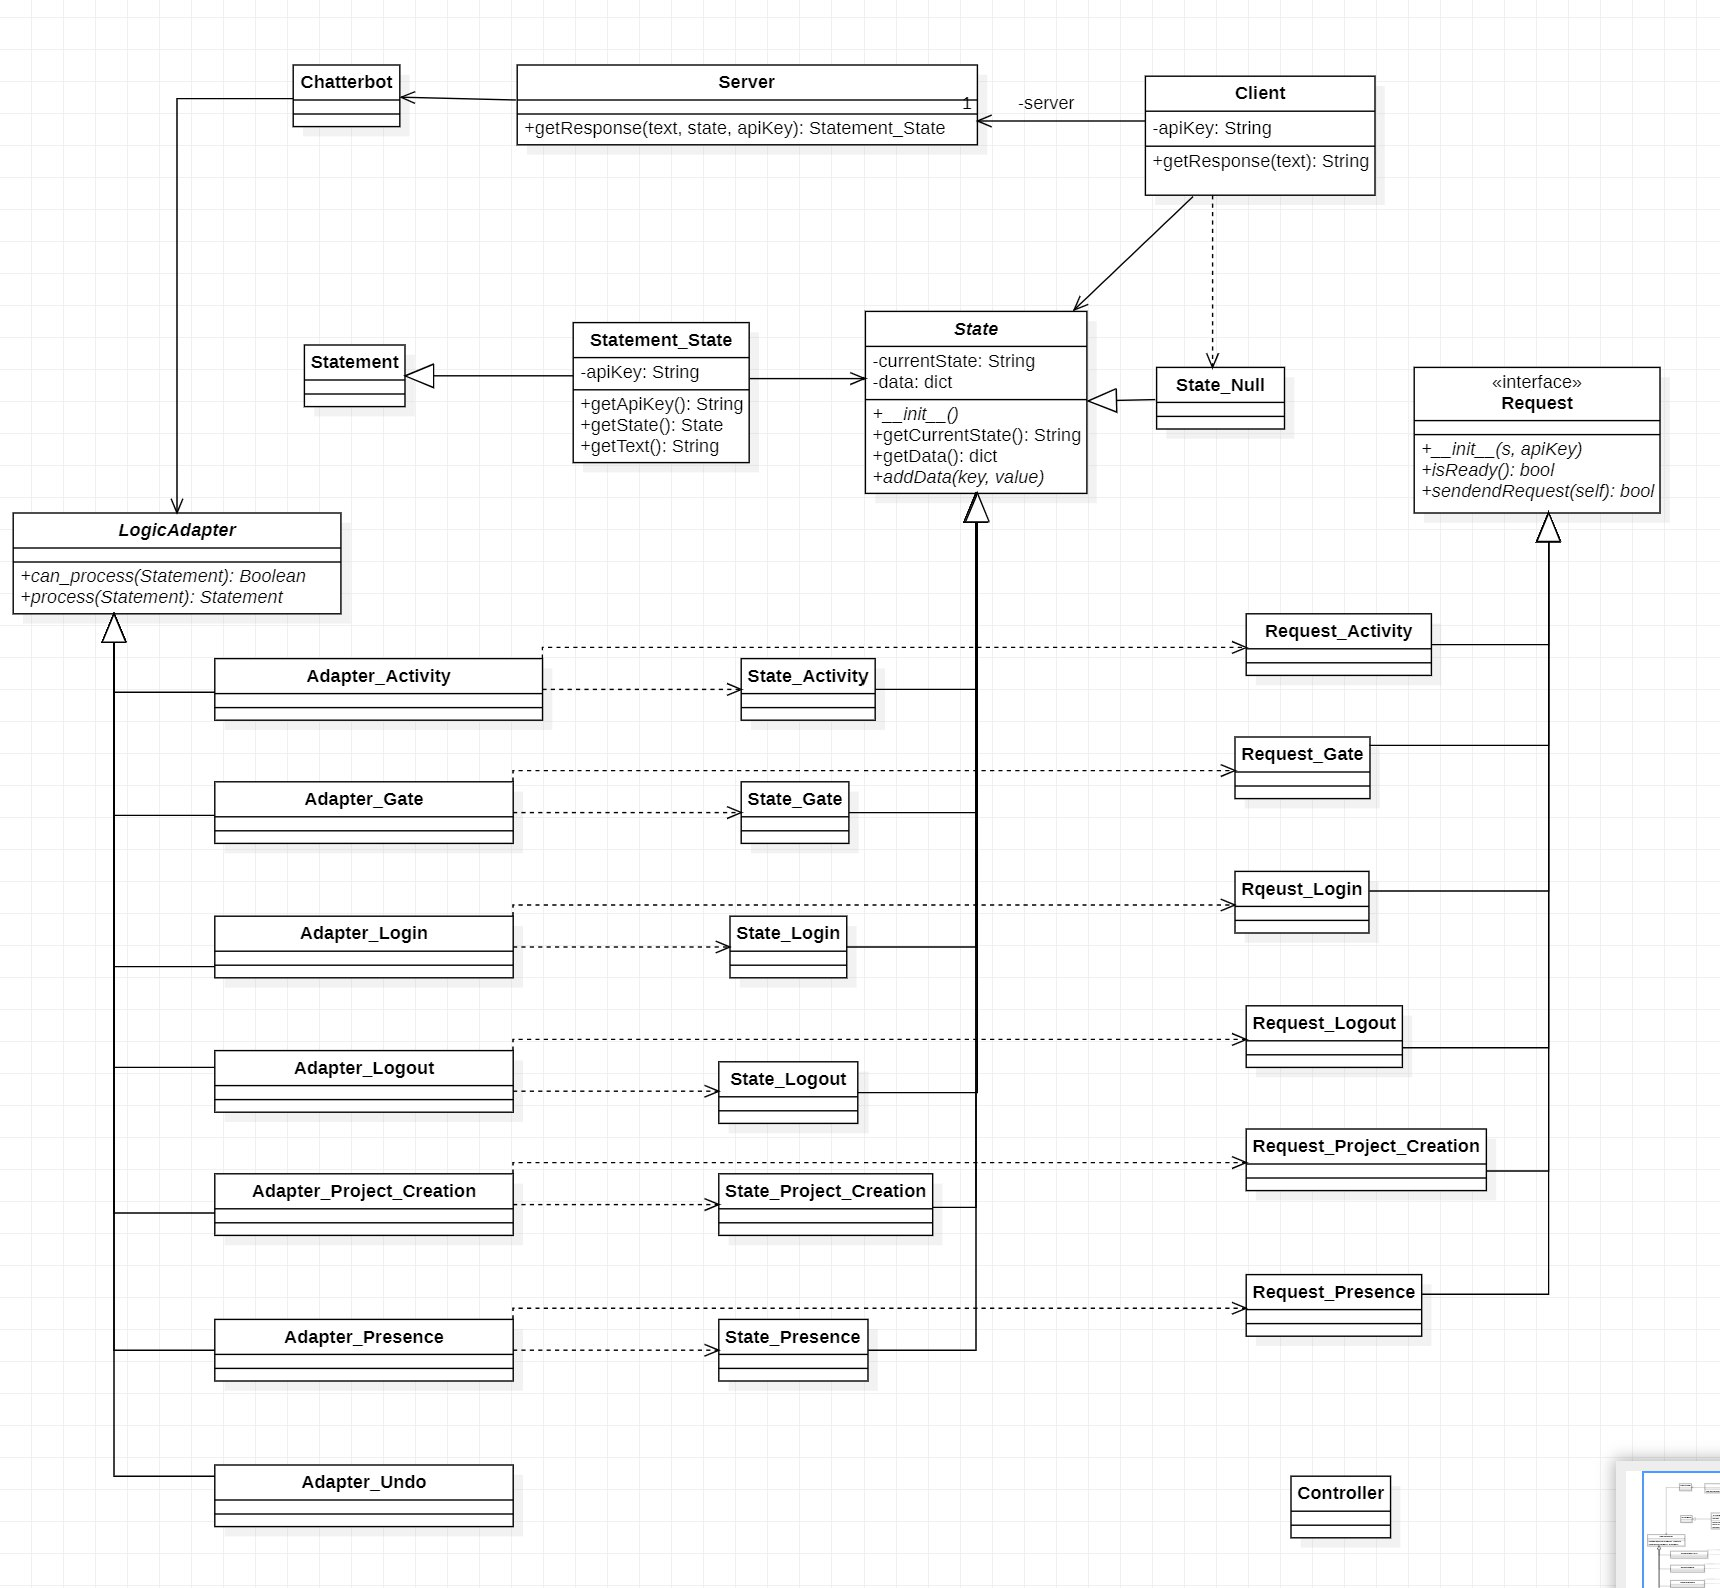
\includegraphics[scale=0.70]{images/diagramma_classi.jpg}
    \caption{Diagramma UML delle classi lato Server}
	\end{figure}

\newpage

\subsection{Server}
\subsubsection{App} Classe in cui vengono gestiti gli utenti e si interfaccia direttamente con l'utente, inoltre assegna il nuovo client id ai nuovi utenti.
\subsubsection{Client} Classe che rappresenta la minisessione di ogni utente nel server e ha tutti i dati salvati.
\subsubsection{Server} Classe che contiene la logica utilizzata dal chatbot per poter rispondere correttamente all'input del client tramite l'utilizzo di \textit{Statement\_State}.
\subsubsection{Chatterbot} Classe della libreria esterna scritta in \glossario{Python}. La classe \textit{Chatterbot} e le seguenti \textit{Statement}, \textit{Adapter} fanno parte della libreria.
\subsubsection{Statement} Classe fornita dalla libreria \glossario{Chatterbot} che rappresenta una singola entità, parola o frase che qualcuno può dire.
\subsubsection{LogicAdapter} Classe astratta fornita dalla libreria \glossario{Chatterbot} che permette al programmatore esterno di scrivere nuovi adapter. Dispone dei due metodi base di cui verrà fatto l'\glossario{overriding}:
    \begin{itemize}
        \item can\_process: metodo booleano che controlla tutte le varie condizioni e se tutto okay fa procedere il metodo \textit{process}.
        \item process: controlla ed elabora tutti i dati forniti così da produrre una risposta.
    \end{itemize}
\subsubsection{State} Interfaccia che definisce il contratto di tutti i vari stati e come dato privato si salva l'attuale stato corrente e pubblicamente dispone anche di un metodo per aggiungere informazioni necessarie per completare la richiesta in corso.
\paragraph*{State\_Null} Sottoclasse concreta di \textit{Stato} che simula uno stato nullo, utilizzato quando l'utente non ha effettuato nessuna richiesta.
\subsubsection{Statement\_State} Sottoclasse di Statement, cioè adatta l'adapter alla libreria chatterbot, in più ha lo stato attuale dell'utente, e l'api-key che dimostra l'autenticazione dell'utente che funge come input di ogni adapter.
\subsubsection{Request} Interfaccia che riceve i dati pronti verificandone la completezza e in base all'\textit{adapter} invia la richiesta \glossario{HTTP} alle \glossario{API Rest} di Imola per interagire con i loro servizi e soddisfare la richiesta dell'utente e infine ritorna ad adapter una risposta.
\subsubsection{Login} Classi \textit{Adapter\_Login}, \textit{State\_Login} permettono di effettuare il login
\subsubsection{Logout} Classe \textit{Adapter\_Logout} permette di effettuare il logout.
\subsubsection{Activity} Classi \textit{Adapter\_Activity}, \textit{State\_Activity} e \textit{Request\_Activity} per la funzionalità di consuntivare le ore dedicate ad un progetto compreso le eventuali ore di viaggio.
\subsubsection{Gate} Classi \textit{Adapter\_Gate}, \textit{State\_Gate} e \textit{Request\_Gate} per la funzionalità di apertura cancello
\subsubsection{Project\_Creation} Classi \textit{Adapter\_Project\_Creation}, \textit{State\_Project\_Creation} e \textit{Request\_Project\_Creation}
\subsubsection{Presence} Classi \textit{Adapter\_Presence}, \textit{State\_Presence} e \textit{Request\_Presence} per la funzionalità di registrazione della presenza
\subsubsection{Undo} Classe \textit{Adapter\_Undo} permette di annullare l'operazione in corso e di ricominciare la stessa o un'altra operazione dall'inizio.
\subsection{Diagramma sequenza Esecuzione Richiesta}
\newpage

\begin{landscape}
	\begin{figure}[H]
	\centering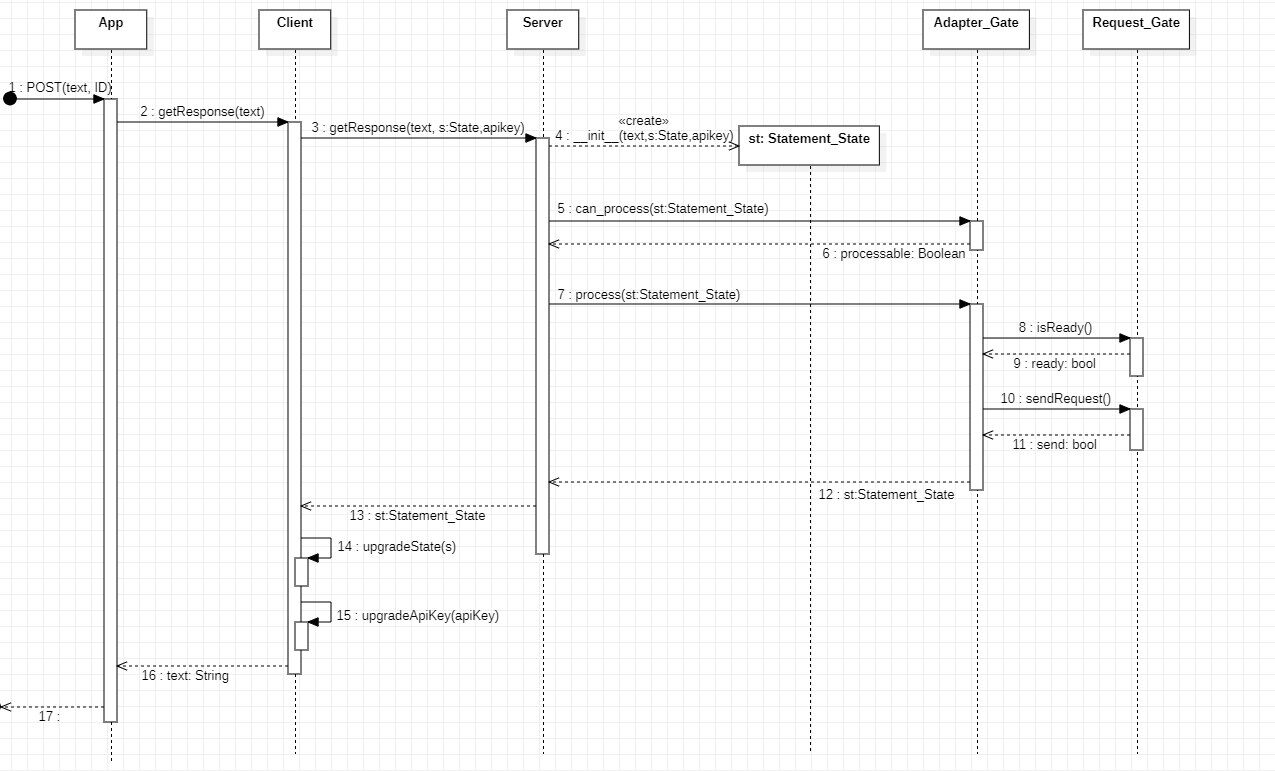
\includegraphics[width=\linewidth]{images/diagramma_sequenza_server.jpg}
    \caption{Diagramma di sequenza Esecuzione Richiesta }
	\end{figure}
\end{landscape}

\subsection{Diagramma sequenza Richiesta Identificativo}
\begin{figure}[H]
    \centering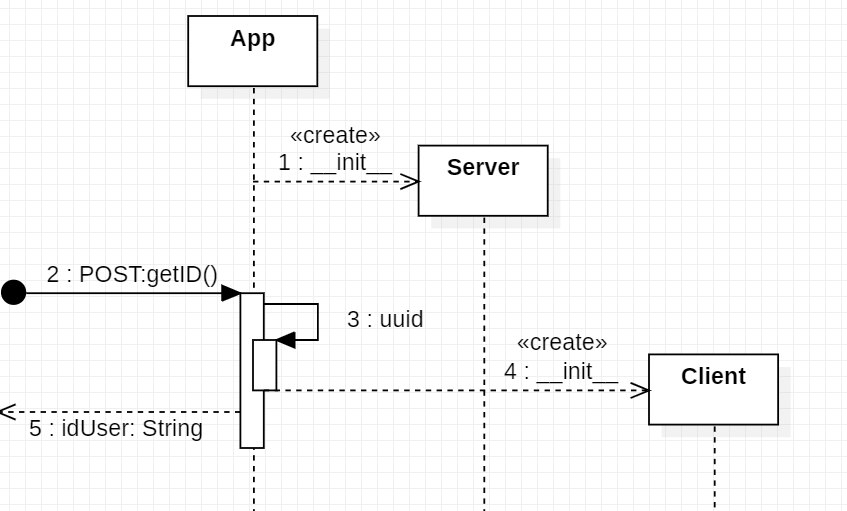
\includegraphics[width=\linewidth]{images/diagramma_sequenza_client.jpg}
    \caption{Diagramma di sequenza Client}
\end{figure}
All'avvio dell'applicazione, il \glossario{Client} ovvero l'interfaccia realizzata tramite \glossario{React}, invia una richiesta di ottenimento dell'identificativo. App, ovvero la classe in cui è instaziato Flask e che si occupa della gestione delle comunicazioni, riceve la richiesta, istanzia una classe Client, lato server, che manterrà in memoria. Questa classe Client, lato server, viene associata ad un \glossario{UUID} in questo modo ogni messaggio successivo mandato dall'utente sarà associato alla sua istanza di classe Client, fino a quando non deciderà di effettuare il logout o gli verrà assegnato un identificativo differente. 

\newpage

\subsection{Design Pattern}
Front Controller pattern è un pattern architetturale per la progettazione di applicazioni web che forniscono un punto di ingresso centralizzato per la gestione delle richieste. Nel caso del nostro applicativo infatti la classe \textit{App}, in cui è presente \glossario{Flask} si occupa di ricevere tutte le richieste ricevute dai vari \glossario{Client}, le quali verranno poi gestite da un'istanza della classe \textit{Client} lato \glossario{Server} che andrà a contattare l'adapter corretto in base all'interpretazione del messaggio, effettuando in seguito una chiamata all'API-REST consona al servizio richiesto.
\newpage

\subsection{API Rest Imola Informatica} L'azienda ha fornito delle \glossario{API Rest} che permettono al \glossario{chatbot} di interagire con i loro sistemi aziendali. Sono facilmente consultabili a questo \href{https://apibot4me.imolinfo.it/}{\color{blue} link}.
\subsubsection{Consuntivazione di un attività}
\paragraph{API Url} \hfill \break
/projects/\{code\}/activities/me
\paragraph{Metodo di richiesta \glossario{HTTP}} \hfill \break
POST
\paragraph{Headers \glossario{HTTP}}
\begin{itemize}
    \item \textbf{accept}: application/json;
    \item \textbf{api\_key}: api\_key, per autorizzare le richieste;
    \item \textbf{Content-Type}: application/json.
\end{itemize}
\paragraph{Parametri URL} \hfill \break
\begin{center}
    \renewcommand{\arraystretch}{1.8}
    \begin{tabular}{ |m{10em}|m{4em}|m{20em}| }
        \hline
        \textbf{Nome} & \textbf{Tipo} & \textbf{Descrizione} \\
        \hline
        code & string & rappresenta il codice del progetto di cui fa parte l’attività da rendicontare.\\
        \hline
    \end{tabular}
\end{center}
\paragraph{Parametri Body} \hfill \break
Nel body della richiesta viene passato un array contenente un json con questi parametri
\begin{center}
    \renewcommand{\arraystretch}{1.8}
    \begin{tabular}{ |m{10em}|m{4em}|m{20em}| }
        \hline
        \textbf{Nome} & \textbf{Tipo} & \textbf{Descrizione} \\
        \hline
        date & string & data in cui si è svolta l'attività.\\
        \hline
        billableHours & int & ore fatturabili dell'attività.\\
        \hline
        travelHours & int & ore di viaggio spese per l'attività.\\
        \hline
        billableTravelHours & int & ore di viaggio fatturabili per l'attività.\\
        \hline
        location & string & nome della sede in cui si è svolta l'attività.\\
        \hline
        billable & bool & indica se l'attività è fatturabile.\\
        \hline
        note & string & descrizione dell'attività.\\
        \hline
    \end{tabular}
\end{center}
\paragraph{Risposte}
\begin{center}
    \renewcommand{\arraystretch}{1.8}
    \begin{tabular}{ |m{9em}|m{24em}| }
        \hline
        \textbf{Status code \glossario{HTTP}} & \textbf{Descrizione} \\
        \hline
        204 & indica che la richiesta di consuntivazione è andata a buon fine\\
        \hline
        404 & indica che il codice specificato del progetto non è corretto\\
        \hline
        401 & indica che l'api key non è stata specificata o quella utilizzata non è valida.\\
        \hline
    \end{tabular}
\end{center}
\subsubsection{Apertura del cancello}
\paragraph{API Url} \hfill \break
/locations/\{location\_name\}/devices/\{device\}/status
\paragraph{Metodo di richiesta \glossario{HTTP}} \hfill \break
PUT
\paragraph{Headers \glossario{HTTP}}
\begin{itemize}
    \item \textbf{accept}: application/json;
    \item \textbf{api\_key}: api\_key, per autorizzare le richieste;
    \item \textbf{Content-Type}: application/json.
\end{itemize}
\paragraph{Parametri URL} \hfill \break
\begin{center}
    \renewcommand{\arraystretch}{1.8}
    \begin{tabular}{ |m{10em}|m{4em}|m{20em}| }
        \hline
        \textbf{Nome} & \textbf{Tipo} & \textbf{Descrizione} \\
        \hline
        location\_name & string & sede di cui aprire il cancello.\\
        \hline
        device & string & nome del dispositivo da utilizzare, in questo caso il cancello.\\
        \hline
    \end{tabular}
\end{center}
\paragraph{Parametri Body} \hfill \break
Nel body della richiesta viene passato un json contenente questi parametri
\begin{center}
    \renewcommand{\arraystretch}{1.8}
    \begin{tabular}{ |m{10em}|m{4em}|m{20em}| }
        \hline
        \textbf{Nome} & \textbf{Tipo} & \textbf{Descrizione} \\
        \hline
        status & string & rappresenta il nuovo stato del dispositivo.\\
        \hline
    \end{tabular}
\end{center}
\paragraph{Risposte}
\begin{center}
    \renewcommand{\arraystretch}{1.8}
    \begin{tabular}{ |m{9em}|m{24em}| }
        \hline
        \textbf{Status code \glossario{HTTP}} & \textbf{Descrizione} \\
        \hline
        204 & indica che la richiesta di apertura del cancello è andata a buon fine.\\
        \hline
        404 & indica che la sede di cui aprire il cancello non è valida.\\
        \hline
        401 & indica che l'api key non è stata specificata o quella utilizzata non è valida.\\
        \hline
    \end{tabular}
\end{center}
\subsubsection{Registrazione della presenza}
\paragraph{API Url} \hfill \break
/locations/\{location\_name\}/presence
\paragraph{Metodo di richiesta \glossario{HTTP}} \hfill \break
POST
\paragraph{Headers \glossario{HTTP}}
\begin{itemize}
    \item \textbf{accept}: application/json;
    \item \textbf{api\_key}: api\_key, per autorizzare le richieste;
    \item \textbf{Content-Type}: application/json.
\end{itemize}
\paragraph{Parametri URL} \hfill \break
\begin{center}
    \renewcommand{\arraystretch}{1.8}
    \begin{tabular}{ |m{10em}|m{4em}|m{20em}| }
        \hline
        \textbf{Nome} & \textbf{Tipo} & \textbf{Descrizione} \\
        \hline
        location\_name & string & sede in cui registrare la presenza.\\
        \hline
    \end{tabular}
\end{center}
\paragraph{Risposte}
\begin{center}
    \renewcommand{\arraystretch}{1.8}
    \begin{tabular}{ |m{9em}|m{24em}| }
        \hline
        \textbf{Status code \glossario{HTTP}} & \textbf{Descrizione} \\
        \hline
        200 & indica che la registrazione della presenza è stata effettuata con successo.\\
        \hline
        404 & indica che la sede specificata non è valida.\\
        \hline
        401 & indica che l'api key non è stata specificata o quella utilizzata non è valida.\\
        \hline
    \end{tabular}
\end{center}
\subsubsection{Creazione di un nuovo progetto}
\paragraph{API Url} \hfill \break
/projects
\paragraph{Metodo di richiesta \glossario{HTTP}} \hfill \break
POST
\paragraph{Headers \glossario{HTTP}}
\begin{itemize}
    \item \textbf{accept}: application/json;
    \item \textbf{api\_key}: api\_key, per autorizzare le richieste;
\end{itemize}
\paragraph{Parametri Body} \hfill \break
Nel body della richiesta viene passato un json contenente questi parametri
\begin{center}
    \renewcommand{\arraystretch}{1.8}
    \begin{tabular}{ |m{10em}|m{4em}|m{20em}| }
        \hline
        \textbf{Nome} & \textbf{Tipo} & \textbf{Descrizione} \\
        \hline
        code & string & codice del progetto da creare.\\
        \hline
        detail & string & descrizione del progetto da creare.\\
        \hline
        customer & string & cliente per cui viene creato il progetto.\\
        \hline
        manager & string & manager del progetto da creare.\\
        \hline
        status & string & stato del progetto.\\
        \hline
        area & string & sede in cui svolgere il progetto.\\
        \hline
        startDate & string & data di inizio del progetto.\\
        \hline
        endDate & string & data di fine del progetto.\\
        \hline
    \end{tabular}
\end{center}
\paragraph{Risposte}
\begin{center}
    \renewcommand{\arraystretch}{1.8}
    \begin{tabular}{ |m{9em}|m{24em}| }
        \hline
        \textbf{Status code \glossario{HTTP}} & \textbf{Descrizione} \\
        \hline
        204 & indica che è l'operazione di creazione del progetto è andata a buon fine.\\
        \hline
        400 & indica che almeno uno dei parametri non è stato specificato.\\
        \hline
        401 & indica che l'api key non è stata specificata o quella utilizzata non è valida.\\
        \hline
    \end{tabular}
\end{center}
\subsubsection{Recupero delle sedi}
\paragraph{API Url} \hfill \break
/locations
\paragraph{Metodo di richiesta \glossario{HTTP}} \hfill \break
GET
\paragraph{Headers \glossario{HTTP}}
\begin{itemize}
    \item \textbf{accept}: application/json;
    \item \textbf{api\_key}: api\_key, per autorizzare le richieste;
\end{itemize}
\paragraph{Risposte}
\begin{center}
    \renewcommand{\arraystretch}{1.8}
    \begin{tabular}{ |m{9em}|m{24em}| }
        \hline
        \textbf{Status code \glossario{HTTP}} & \textbf{Descrizione} \\
        \hline
        200 & ritorna una lista contenente le informazioni delle sedi.\\
        \hline
        401 & indica che l'api key non è stata specificata o quella utilizzata non è valida.\\
        \hline
    \end{tabular}
\end{center}
\subsubsection{Recupero della rendicontazione per il progetto corrente}
\paragraph{API Url} \hfill \break
/projects/\{code\}
\paragraph{Metodo di richiesta \glossario{HTTP}} \hfill \break
GET
\paragraph{Headers \glossario{HTTP}}
\begin{itemize}
    \item \textbf{accept}: application/json;
    \item \textbf{api\_key}: api\_key, per autorizzare le richieste;
\end{itemize}
\paragraph{Parametri URL} \hfill \break
\begin{center}
    \renewcommand{\arraystretch}{1.8}
    \begin{tabular}{ |m{10em}|m{4em}|m{20em}| }
        \hline
        \textbf{Nome} & \textbf{Tipo} & \textbf{Descrizione} \\
        \hline
        code & string & codice del progetto corrente.\\
        \hline
    \end{tabular}
\end{center}
\paragraph{Risposte}
\begin{center}
    \renewcommand{\arraystretch}{1.8}
    \begin{tabular}{ |m{9em}|m{24em}| }
        \hline
        \textbf{Status code \glossario{HTTP}} & \textbf{Descrizione} \\
        \hline
        200 & ritorna un json contenente le informazioni per il progetto corrente.\\
        \hline
        401 & indica che l'api key non è stata specificata o quella utilizzata non è valida.\\
        \hline
    \end{tabular}
\end{center}

